\section{The Serverless Edge Platform}\label{sec:SEP}

\subsection{Mobile Computation Offloading}\label{sec:SEP_MCO}

The offloading of computation from mobile devices to cloud servers was firstly addressed by the concept of Mobile Cloud Computing~\cite{Khan:14}. Its main purpose was to enable rich mobile applications to be executed in resource-constrained mobile devices. However, this approach is limited by network latency, which is prohibitive for most real-time and interactive applications.

Addressing the network latency problem, \textit{cloudlets}~\cite{Satyanarayanan:2009} --- a precursor of edge computing --- have been proposed as resource-rich computer or cluster of computers  accessible through wireless local area network (WLAN). Their purpose is to enable the offloading of latency-sensitive computation from mobile and, more recently, general IoT devices. 

%To address this kind of edge computing scenario, an edge platform should support the execution of \textit{latency-sensitive} tasks. With the evolution of mobile devices capabilities, \textit{computing-intensive} tasks from real-time applications are of particular interest.

To illustrate this scenario, let us consider an Augemented Reality (AR) application that relies on two tasks: one for \textit{feature extraction} and another for \textit{feature matching}. The first handles the extraction of features from captured video frames, whilst the second matches theses features against a catalog (e.g., points of interest in a city area). 
%By offloading these tasks to a surrogate edge platform, the application is able to recognize more POIs while avoiding to stress the mobile device.
These computation-intensive, latency-sensitive tasks are strong candidates for been offloaded from hosting devices.

Targeting these requirements, a serverless edge platform (SEP) can exploit the FaaS model to allow tasks such as the \textit{feature extraction} and \textit{matching} to be written as stateless functions and consumed as web services. The resulting architecture would consist of two independent, fine-grained and highly cohesive FaaS-based services\footnote{We do not use the microservice terminology despite the characteristics of that FaaS-based services share with microservices}. Alternatively, both functions could compose a single, coarser service. Its main advantage would be the reduced communication overhead. However, in the context of edge computing, separating functions into distinct services has the following benefits: i) it allows different functions to be consumed independently by distinct applications (e.g., a common feature extracting service); and ii) it allows functions to be deployed and scaled independently.%; and iii) it allows the dynamic placement of functions into different edge and cloud platforms.

The last advantage is particularly important, as different types of edge infrastructures~\cite{Satyanarayanan:2009,Taleb:2013,Liu:2014,K.Wang:2015} converge in one aspect: their limitation of computational resources. The separation of functions with different responsibilities and requirements into independent services allows each function to be provided by distinct edge platforms; the decision of where to execute each function will depend on factors such as the characteristics and requirements of each function, the capabilities of distinct edge platforms, and the network latency and throughput among edge platforms and client devices. In a hierarchical topology~\cite{Liu:2014}, data-intensive functions are best candidates for been placed in close proximity to the edge, whereas computing-intensive functions may require more powerful resources from intermediary edge nodes. 

Figure~\ref{fig:Mobile_Computation_Offloading_F1} depicts the two AR functions as a single service (one request per offloading), whilst Figure~\ref{fig:Mobile_Computation_Offloading_F2} depicts each function as an independent service (two requests per offloading). 
In the first approach, mobile devices (md) connected to SEP A are unable to offload computation, as the fEM function is currently unavailable at that platform and the network throughput among these SEPs is insufficient for delegating requests with a video frame payload.
In the second approach, data-intensive \textit{feature extraction} (fE) is performed by both SEPs. Conversely, \textit{feature matching} (fM) is unavailable at SEP A; fM requests targeting this platform are offloaded to SEP B by its \textit{Load Balancer},
%or to the cloud by a load balancer, 
thanks to the reduced payload size (frame features extracted by fE) and the low latency among these surrogate platforms. 



%First, the FaaS model is based on events; 

\begin{figure}[tbp]
	\centering
	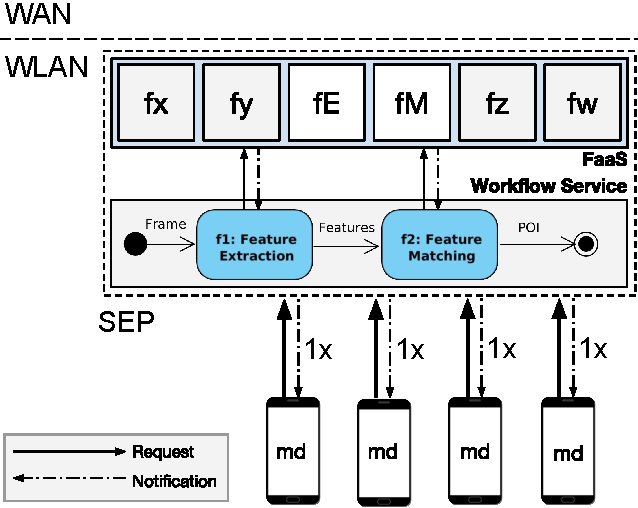
\includegraphics[width=\linewidth]{Figs/Mobile_Computation_Offloading_Workflow.pdf}
	\caption{An AR workflow involving the sequential execution of the \textit{feature extraction} (fE) and \textit{feature matching} (fM) functions; each video frame generates a single (1x) request, which is processed by one instance of each function.} 
	\label{fig:Mobile_Computation_Offloading_Workflow}
\end{figure}

Notwithstanding the benefits of the FaaS model, the satisfaction of low-latency requirements by the serverless edge platform requires further optimization.

%In the FaaS model
First, functions are externally triggered by HTTP requests. In the context of real-time applications, communication overhead must be kept minimal. As such, the edge platform must include an interface that allows clients to trigger sequential or parallel execution of functions composing different services without the overhead associated to the HTTP protocol. In this regard, the \textit{WebSocket protocol}~\footnote{https://tools.ietf.org/html/rfc6455}
%is a standardized protocol that 
provides full-duplex communication channels over a single TCP connection. %Figure~\ref illustrates this feature.

%For this, each task is deployed as a stateless, fully-managed function and exposed as a web service. 
%Within milliseconds, the fully-managed platform allocates a containerized runtime instance in which the function is first executed, whereas subsequent executions may take advantage of existing instances.
%Dependencies, if any, are described within a package descriptor and made available by the platform.
%Finally, a third function gets detailed information about each POI from a remote database.
%In particular, OpenWhisk is an state-of-art and open source FaaS platform.

The support for websockets would enable real-time interactions between mobile clients and the edge platform. Still, individual function invocations may add significant latency overhead whenever two or more functions form an execution flow. To avoid this overhead, developers would be forced to either chain function calls through hardcoded dependencies, or write coarser and less cohesive functions. Moreover, the chaining of function also imposes a cost overhead, since calling functions are kept waiting.% for other function(s) to return. 

To address latency, design, cost, and resource efficiency concerns, the SEPs should support \textit{function workflows}. This kind of service would allow developers to define, through visual or textual programming, a function execution flow.
%starting with the processing of the input sent by a client and finishing with the result sent back to the client. 
Similarly to functions, workflows are triggered by events; at each intermediary step, result from one function is passed to the subsequent function call. Going back to the AR example, Figure~\ref{fig:Mobile_Computation_Offloading_Workflow} depicts a simple workflow consisting of the sequential execution of the \textit{feature extraction} and \textit{matching} functions, which remain decoupled.% of each other.

\begin{figure}[tbp]
	\centering
	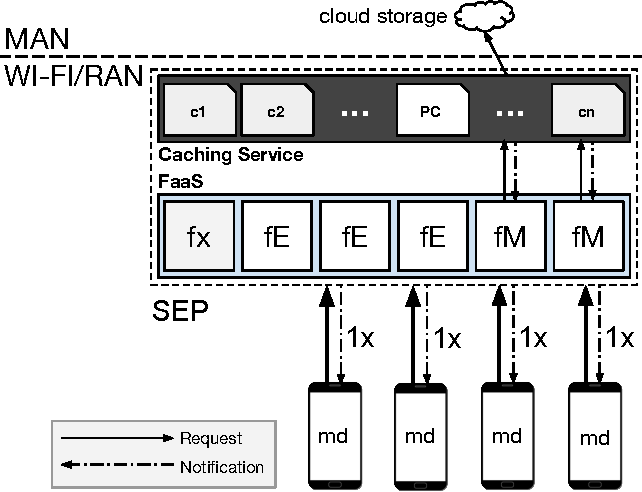
\includegraphics[width=\linewidth]{Figs/Mobile_Computation_Offloading_Caching.pdf}
	\caption{A SEP with three instances of the \textit{feature extraction} (fE) and two instances of the \textit{feature matching} (fM) functions; a local copy of the POI catalog (PC) is fetched once from a cloud storage service and served to the fM instances.} 
	\label{fig:Mobile_Computation_Offloading_Caching}
\end{figure}

Last but not least, existing FaaS platforms (e.g., AWS Lambda and Apache OpenWhisk) enforce a programming model in which functions have access to a transient folder without guaranteeing that subsequent invocations will be executed by the same containerized environment. %Thus, each invocation must check whether cached data is available. 
In the context of real-time applications, retrieving extensive data sets may add prohibitive overhead. For instance, in the AR example, a POI catalog (circa 1Gb) is employed to identify points of interest against their matched features. Due to size limitations, it can not be packed with the function source code, but needs to be retrieved dynamically.
%Cloud vendors provide storage services as part of their platform ecosystem. 

%TODO: make it consistent with the PROTOTYPE Section
%To address the need of edge services with dependency to large data sets
Addressing the aforementioned issue, we propose to equip SEPs with a caching service. This service should fetch data from cloud-based storage services and keep it available locally for mitigating networking overhead. 
%More precisely, it consists of an object-based storage system, in which files are associated with metadata. 
To make use of this service, SEP functions request files passing their cloud URI, which should return a valid file format.
% --- and an optional expiration policy. 
Once retrieved, the caching service stores the file along with the metadata containing its URI and frequency of access; subsequent requests are served without networking overhead. 
Figure~\ref{fig:Mobile_Computation_Offloading_Caching} illustrates the interplay between the caching service storing a POI catalog (PC) retrieved from a cloud storage and multiple runtime instances of the \textit{feature matching} function.

%TODO: move this to the prototype section?
%To support different kinds of edge infrastructure, the SEP caching service should rotate cached files according to the availability of storage resources and the access frequency of cached files. As such, files accessed less frequently are subject for been replaced in case of resource contention. 
%%Files without an expiration date are replaced only in case of resource contention following the access frequency policy. 


%A serverless edge platform should support a more efficient caching service to optimize use cases in which functions have data dependencies. 
\subsection{Edge Data Analysis}

\begin{figure}[tbp]
	\centering
	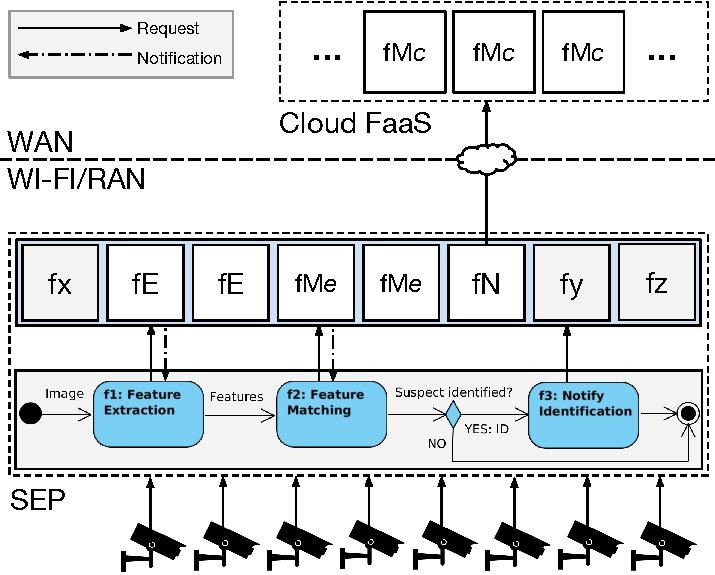
\includegraphics[width=\linewidth]{Figs/Edge_Data_Analytics_Video_Surveillance.pdf}
	\caption{Features from video frames captures by surveillance cameras are extracted (fE) and, upon a positive matching (fM$e$), sent for further analysis by a cloud service (fM$c$).}
	\label{fig:Edge_Data_Analytics_Video_Surveillance}
\end{figure}

More recently, the advent of data-intensive Internet of Things (IoT) devices and applications raised concerns about the feasibility of sending exponentially larger volumes of data through the Internet all the way to cloud data centres. Accordingly, another important motivation for edge computing consists of the anticipation of the analysis of data produced and consumed by applications at the network edge. 

%TODO: find an example with low-latency requirement?
%Differently from the mobile computation offloading scenario, the most important concerns of edge data analysis are network throughput 
%(to cope with large volumes of data) 
%and preventing network bottlenecks caused by centralization. Still, edge analysis may also need to cope with low-latency requirements, specially if analysis results should feed latency-sensitive actuation.

%To illustrate this scenario
For example, in the context of smart cities and cyber-physical-systems, let us consider a video surveillance application depicted by Figure~\ref{fig:Edge_Data_Analytics_Video_Surveillance}. Similarly to the AR application, compute-intensive functions such as \textit{feature extraction} (fE) and \textit{matching} (fM\textit{e}) are assigned to edge platforms.
%, this time with the purpose of recognizing faces from a police catalog. 
These functions compose a workflow exposed as a service and consumed by resource-constrained IoT cameras. This service receives video frames at short intervals, from which it extracts facial features matched against a police catalog (PC). A positive identification triggers the execution of a cloud-based service (fM\textit{c}) responsible for a more robust analysis able to detect false positives. In this manner, large volumes of data are processed at the edge, preventing the congestion of the wide area network (WAN) and the centralized services.



Still in the context of edge data analysis, 
%other use cases exhibit more strict requirements for latency. For instance, 
let us imagine that in the future the majority of elderly citizen will be wearing body sensors to collect data about their health status. In the event of an anomalous condition (e.g., the beginning of a heart attack), emergency services should be dispatched immediately to the person location. Moreover, it is very important to provide the person with feedback so she can ask nearby people for their assistance.
%other people that can provide a first and immediate assistance.
%The IoT-based heart disease monitoring system for pervasive healthcare service
The accurate identification of such events, however, requires complex analysis of data from different sensors (e.g., heart rate, oxigen saturation, glucose~\cite{Li:2017}). Offloading the analysis from all users to the cloud may overload the network and centralized services. Instead, this burden should be shared with SEPs.% composing the mobile networks infrastructure (e.g., base stations, multi-technology aggregation sites, etc~\cite{}). 

The aforementioned examples share one characteristic: their main purpose is to prevent large volumes of data to be sent and processed by distant data centres. In the latter example, providing feedback in a timely manner is important, but does not fall into the category of low ($\leq 100ms$) or ultra-low ($\leq 20ms$) latency requirements. For this kind of application, the offloading of data analysis from the cloud to the edge should be opportunistic and informed by the availability of computing and networking resources, as well as the characteristics and requirement of each function.

As discussed in Section~\ref{sec:SEP_MCO}, the proposed architecture (see Figure~\ref{fig:Mobile_Computation_Offloading}) enables fine-grained functions to be placed onto different platforms, including cloud-based FaaS. This dynamic decision can be either orchestrated by a centralized entity~\cite{Taleb:2013}, coordinated among different edge and cloud platforms~\cite{Mach:2017}, and involve the participation of client devices~\cite{Baresi:2018}. Based on a given placement scheme, an informed \textit{Load Balancer} makes the timely decision on the destination of each request arriving at its own SEP.



%Differently from the mobile computation offloading scenario, edge data analysis may tolerate higher delays, in which case a \textit{scheduler} should decide between edge-based and cloud-based services. 

\begin{figure}[tbp]
	\centering
	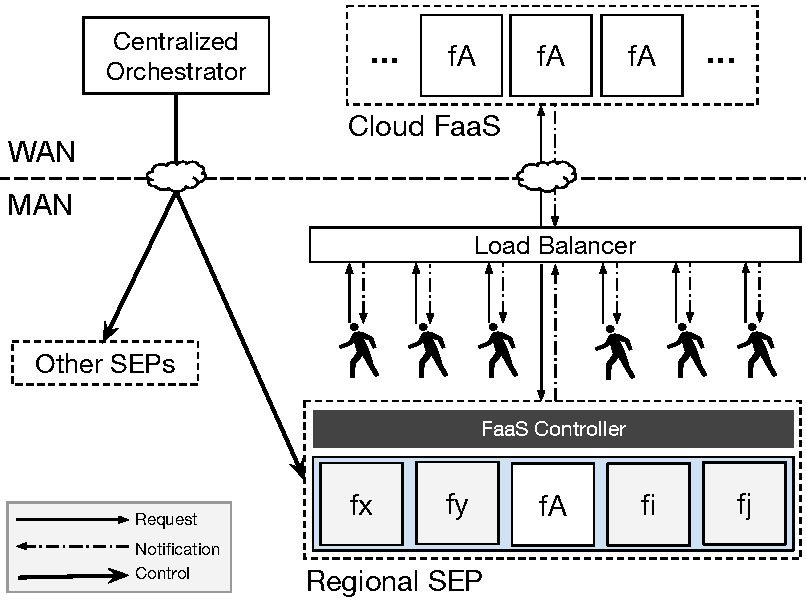
\includegraphics[width=\linewidth]{Figs/Edge_Data_Analytics_Personal_Assistant.pdf}
	\caption{Instances of the \textit{health analysis} function (fA) are placed to SEPs by a centralized \textit{Orchestrator}; given the current placement scheme, a \textit{Load Balancer} distributes requests among its local FaaS and the cloud-based FaaS based on the fA requirement for latency and the average response time.}
	\label{fig:Edge_Data_Analytics_Personal_Assistant}
\end{figure}

Figure~\ref{fig:Edge_Data_Analytics_Personal_Assistant} presents the opportunistic placement of a \textit{health analysis} function (fA) onto edge and cloud platforms. Based on the availability of resources at each SEP and the demand for different functions, a \textit{Centralized Orchestrator} decides for the number of runtime instances for each function with the goal of optimizing the allocation of SEP resources. Informed of this decision, a \textit{Load Balancer} assigns incoming requests to its local FaaS or to the cloud-based FaaS, taking into account the latency requirement and the average response time. 

Still in the same example, upon a heath emergency the fA function proceeds with two actions: i) the invocation of an external emergency service; and ii) the notification of the personal assistant device about the emergency. For this, the \textit{Load Balancer} must also work as a \textit{reverse proxy} to assure results will be sent back to personal assistance devices regardless of the platform each request have been assigned to.

%In particular, the scheduling should take into account the latency constraints of each type of service.

%For instance, let us consider the case of a mobile crowd sensing application in which environmental data (e.g., air pollution~\footnote{a common type of sensor in smartphones in China}) is collected from sensors embedded in smartphones, tablets, and variables accompanying people. 

%This example poses one challenge: if functions are stateless and their instances ephemeral, how should the platform deal with long-living cases of data analysis? 

\subsection{Real-time Edge Coordination}

\begin{figure}[tbp]
	\centering
	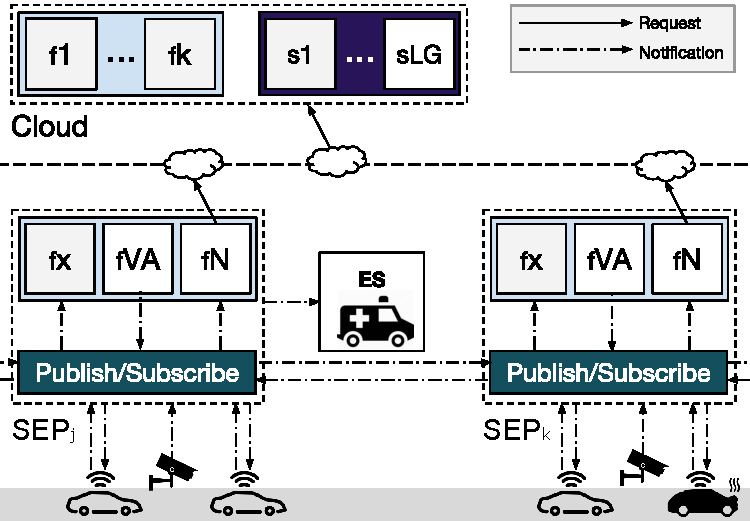
\includegraphics[width=1\linewidth]{Figs/Edge_Coordination_AVs_wide.pdf}
	\caption{Autonomous Vehicles, a road monitoring system, an emergency service and a logging service are coordinated by means of a distributed event bus hosted by surrogated SEPS}
	\label{fig:Edge_Coordination_AVs}
\end{figure}

Another important application scenario involves the real-time coordination among distributed mobile and IoT devices at the network edge. To illustrate this scenario, let us consider the coordination among Autonomous Vehicles (AV). Each vehicle is expected to generate large volumes of data from its sensors, including the AV's actual position, speed, and acceleration. AVs make use of sophisticate mechanisms to prevent collisions. Notwithstanding this, AVs traveling at high speeds would benefit from real-time notifications of anomalous events in their path (e.g., accidents). 

To address real-time coordination among edge devices, SEPs can feature a publish-subscribe (pub-sub) notification service. This service would allow edge devices (e.g., AVs, surveillance cameras) to coordinate with other devices and additional systems integrated with the edge platform (e.g., a road monitoring system). In addition to localized coordination, surrogate SEPs must form a distributed event bus, enabling inter-platform coordination (e.g., AVs and cameras connected to different SEPs). Other edge-based systems (e.g., an emergency service) could also subscribe to anomalous events in order to take actions (e.g., to dispatch ambulances or road patrols) in a timely manner.

The integration enabled by a pub-sub service fits well in a serverless architecture~\cite{Lloyd18serverless}. Indeed, existing FaaS platforms (e.g., AWS Lambda~\cite{AWSLambda}) are integrated with other systems by means of notification services (e.g., AWS SNS) in which functions are triggered by event notifications. In the AV coordination example, a similar approach could be used to trigger, upon an anomalous event, a specific function responsible for the invocation of an external service (e.g., a cloud-based service that persists the occurrence of the anomalous event). 


Figure~\ref{fig:Edge_Coordination_AVs} illustrates the solution for the AVs coordination example. AVs subscribe to the pub-sub service hosted by surrogate SEPs; anomalous events --- reported by AVs or video analysis functions (fE and fM) --- are propagated to the AVs within its own SEP zone, to those behind, and to an emergency service (ES). Finally, a cloud-based logging service (sLG) is invoked by a SEP-based notification function (fN). In order to prevent multiple invocations of the logging service, the notification function at each SEP must distinguish between local events and those from other platforms. The same is valid for the emergency squad service covering different road sections. To satisfy this requirement, the pub-sub service should enforce location-awareness by mapping each event to its SEP of origin.

\subsection{Stateful Edge Services}

One of the most important directives concerning the design of web services is to move state into a separate layer~\cite{Armbrust:2010}. Stateless services are easier to test, debug, and scale, whereas stateful services require state to be recreated for testing and debug purposes, and achieving consistency among replicated instances incur in performance degradation. However, some application scenarios exhibit particular needs that justify the adoption of stateful services.


To illustrate this requirement, let us think of a mobile multiplayer game (MMG). As an interactive application, low-latency is a first class requirement that justifies the deployment of services to the network edge. As an example, \textit{PokemonGO}, a popular MMG, features a single interactive use case in which players interact with virtual \textit{Pokemons}~\footnote{A fantasy creature collected by players} added to their devices screen. 
%

To increase the game popularity, a new interactive feature could enable users in the same city area to start game battles involving their \textit{Pokemons}. Following a conventional multiplayer game architecture, an authoritative service is designed to host the game battle state and business logic. In particular, the state represents a battle session, whilst business logic is responsible for updating the state according to user inputs and other events. 

Addressing the aforementioned example, the solution depicted in Figure~\ref{fig:Steteful_Edge_MMG} exploits two benefits from stateful services: first, it prevents the overhead of transferring to the service, at each user interaction, the whole state of the battle; second, it allows an authoritative service to manage changes to the game state that may not be safely delegated to clients, who otherwise could modify the local game logic and state to their own advantage.
%(e.g., in a P2P architecture)
Composing the rest of the application, other delay-tolerant features (e.g., players scores) should be managed by resourceful, long-living cloud-based services, accessed without SEP inter-mediation. Finally, to prevent the overhead associated with replicated state, stateful instances should be vertically scaled --- with the dynamic allocation of CPU/memory resources --- in detriment of horizontal scaling through instance replication. %Figure~\ref{fig:Steteful_Edge_MMG} depicts the resulting architecture.%; instances of the stateful \textit{multiplayer battle service} are hosted by the serverless edge platform precisely when needed. 

The support for stateful services comes with a cost. To address the specific use cases requiring stateful services, a serverless edge platform should impose limitations. More precisely, stateful services should be designed to last for a limited duration corresponding to the lifetime of a specific latency-sensitive use case. Similarly to its stateless counterpart, it should be created and terminated on demand in a timely manner without preallocating resources.


\begin{figure}[tbp]
	\centering
	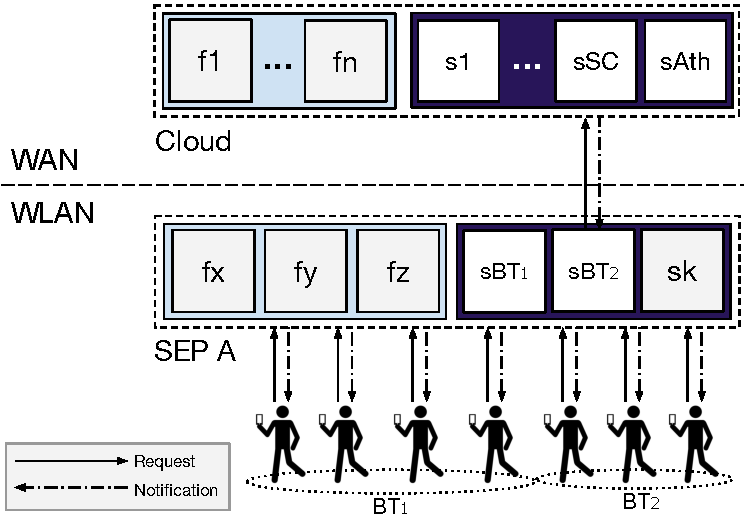
\includegraphics[width=\linewidth]{Figs/Stateful_Edge_Services.pdf}
	\caption{A stateful service enables multiple players to join game battle sessions (BT$_1$, BT$_2$); instances (sBT$_1$, sBT$_2$) are mapped to each session; authentication (sAuth) and player scores (sSC) are managed by cloud-based services.}
	\label{fig:Steteful_Edge_MMG}
\end{figure}


%\subsection{On Premise Edge}

%Serverless computing has been conceived as a cloud model. Notwithstanding this, a serverless architecture can be adopted by on premise edge infrastructure to deliver self-managed services to smart home, office, and Industry 4.0 applications. For this, on premise SEPs should exhibit the computational resources and services (discussed along the present section) compatible with targeted applications. 

%Also, on premise and on demand SEPs can form an infrastructure continuum supporting mobility.

%We conclude the present section with a typical smart home scenario in which a plethora of sensors providehttps://www.overleaf.com/project/5bb1f5b57d8ebf292d2436ed information about the environment and actuators operate on different equipment. Communication with the domestic SEP is performed with lightweight protocols (e.g., COAP~\cite{} and MQTT~\cite{}). Functions are triggered by events (e.g., from sensors), direct calls (e.g., from smart devices) or execution flows (e.g., from a microclimate analysis workflow). Figure~\ref{} illustartes this scenario.
